\documentclass[]{article}
\usepackage{lmodern}
\usepackage{amssymb,amsmath}
\usepackage{ifxetex,ifluatex}
\usepackage{fixltx2e} % provides \textsubscript
\ifnum 0\ifxetex 1\fi\ifluatex 1\fi=0 % if pdftex
  \usepackage[T1]{fontenc}
  \usepackage[utf8]{inputenc}
\else % if luatex or xelatex
  \ifxetex
    \usepackage{mathspec}
  \else
    \usepackage{fontspec}
  \fi
  \defaultfontfeatures{Ligatures=TeX,Scale=MatchLowercase}
\fi
% use upquote if available, for straight quotes in verbatim environments
\IfFileExists{upquote.sty}{\usepackage{upquote}}{}
% use microtype if available
\IfFileExists{microtype.sty}{%
\usepackage{microtype}
\UseMicrotypeSet[protrusion]{basicmath} % disable protrusion for tt fonts
}{}
\usepackage[margin=1in]{geometry}
\usepackage{hyperref}
\hypersetup{unicode=true,
            pdftitle={Basic concepts of Statistics: Inference},
            pdfauthor={Livio Finos},
            pdfborder={0 0 0},
            breaklinks=true}
\urlstyle{same}  % don't use monospace font for urls
\usepackage{color}
\usepackage{fancyvrb}
\newcommand{\VerbBar}{|}
\newcommand{\VERB}{\Verb[commandchars=\\\{\}]}
\DefineVerbatimEnvironment{Highlighting}{Verbatim}{commandchars=\\\{\}}
% Add ',fontsize=\small' for more characters per line
\usepackage{framed}
\definecolor{shadecolor}{RGB}{248,248,248}
\newenvironment{Shaded}{\begin{snugshade}}{\end{snugshade}}
\newcommand{\AlertTok}[1]{\textcolor[rgb]{0.94,0.16,0.16}{#1}}
\newcommand{\AnnotationTok}[1]{\textcolor[rgb]{0.56,0.35,0.01}{\textbf{\textit{#1}}}}
\newcommand{\AttributeTok}[1]{\textcolor[rgb]{0.77,0.63,0.00}{#1}}
\newcommand{\BaseNTok}[1]{\textcolor[rgb]{0.00,0.00,0.81}{#1}}
\newcommand{\BuiltInTok}[1]{#1}
\newcommand{\CharTok}[1]{\textcolor[rgb]{0.31,0.60,0.02}{#1}}
\newcommand{\CommentTok}[1]{\textcolor[rgb]{0.56,0.35,0.01}{\textit{#1}}}
\newcommand{\CommentVarTok}[1]{\textcolor[rgb]{0.56,0.35,0.01}{\textbf{\textit{#1}}}}
\newcommand{\ConstantTok}[1]{\textcolor[rgb]{0.00,0.00,0.00}{#1}}
\newcommand{\ControlFlowTok}[1]{\textcolor[rgb]{0.13,0.29,0.53}{\textbf{#1}}}
\newcommand{\DataTypeTok}[1]{\textcolor[rgb]{0.13,0.29,0.53}{#1}}
\newcommand{\DecValTok}[1]{\textcolor[rgb]{0.00,0.00,0.81}{#1}}
\newcommand{\DocumentationTok}[1]{\textcolor[rgb]{0.56,0.35,0.01}{\textbf{\textit{#1}}}}
\newcommand{\ErrorTok}[1]{\textcolor[rgb]{0.64,0.00,0.00}{\textbf{#1}}}
\newcommand{\ExtensionTok}[1]{#1}
\newcommand{\FloatTok}[1]{\textcolor[rgb]{0.00,0.00,0.81}{#1}}
\newcommand{\FunctionTok}[1]{\textcolor[rgb]{0.00,0.00,0.00}{#1}}
\newcommand{\ImportTok}[1]{#1}
\newcommand{\InformationTok}[1]{\textcolor[rgb]{0.56,0.35,0.01}{\textbf{\textit{#1}}}}
\newcommand{\KeywordTok}[1]{\textcolor[rgb]{0.13,0.29,0.53}{\textbf{#1}}}
\newcommand{\NormalTok}[1]{#1}
\newcommand{\OperatorTok}[1]{\textcolor[rgb]{0.81,0.36,0.00}{\textbf{#1}}}
\newcommand{\OtherTok}[1]{\textcolor[rgb]{0.56,0.35,0.01}{#1}}
\newcommand{\PreprocessorTok}[1]{\textcolor[rgb]{0.56,0.35,0.01}{\textit{#1}}}
\newcommand{\RegionMarkerTok}[1]{#1}
\newcommand{\SpecialCharTok}[1]{\textcolor[rgb]{0.00,0.00,0.00}{#1}}
\newcommand{\SpecialStringTok}[1]{\textcolor[rgb]{0.31,0.60,0.02}{#1}}
\newcommand{\StringTok}[1]{\textcolor[rgb]{0.31,0.60,0.02}{#1}}
\newcommand{\VariableTok}[1]{\textcolor[rgb]{0.00,0.00,0.00}{#1}}
\newcommand{\VerbatimStringTok}[1]{\textcolor[rgb]{0.31,0.60,0.02}{#1}}
\newcommand{\WarningTok}[1]{\textcolor[rgb]{0.56,0.35,0.01}{\textbf{\textit{#1}}}}
\usepackage{graphicx,grffile}
\makeatletter
\def\maxwidth{\ifdim\Gin@nat@width>\linewidth\linewidth\else\Gin@nat@width\fi}
\def\maxheight{\ifdim\Gin@nat@height>\textheight\textheight\else\Gin@nat@height\fi}
\makeatother
% Scale images if necessary, so that they will not overflow the page
% margins by default, and it is still possible to overwrite the defaults
% using explicit options in \includegraphics[width, height, ...]{}
\setkeys{Gin}{width=\maxwidth,height=\maxheight,keepaspectratio}
\IfFileExists{parskip.sty}{%
\usepackage{parskip}
}{% else
\setlength{\parindent}{0pt}
\setlength{\parskip}{6pt plus 2pt minus 1pt}
}
\setlength{\emergencystretch}{3em}  % prevent overfull lines
\providecommand{\tightlist}{%
  \setlength{\itemsep}{0pt}\setlength{\parskip}{0pt}}
\setcounter{secnumdepth}{0}
% Redefines (sub)paragraphs to behave more like sections
\ifx\paragraph\undefined\else
\let\oldparagraph\paragraph
\renewcommand{\paragraph}[1]{\oldparagraph{#1}\mbox{}}
\fi
\ifx\subparagraph\undefined\else
\let\oldsubparagraph\subparagraph
\renewcommand{\subparagraph}[1]{\oldsubparagraph{#1}\mbox{}}
\fi

%%% Use protect on footnotes to avoid problems with footnotes in titles
\let\rmarkdownfootnote\footnote%
\def\footnote{\protect\rmarkdownfootnote}

%%% Change title format to be more compact
\usepackage{titling}

% Create subtitle command for use in maketitle
\providecommand{\subtitle}[1]{
  \posttitle{
    \begin{center}\large#1\end{center}
    }
}

\setlength{\droptitle}{-2em}

  \title{Basic concepts of Statistics: Inference}
    \pretitle{\vspace{\droptitle}\centering\huge}
  \posttitle{\par}
    \author{Livio Finos}
    \preauthor{\centering\large\emph}
  \postauthor{\par}
      \predate{\centering\large\emph}
  \postdate{\par}
    \date{23 October 2019}


\begin{document}
\maketitle

{
\setcounter{tocdepth}{2}
\tableofcontents
}
\hypertarget{outline}{%
\section{Outline}\label{outline}}

\hypertarget{outline-1}{%
\subsection{Outline}\label{outline-1}}

Measuring the dependence among variables:

\begin{itemize}
\tightlist
\item
  Covariance and Correlation\\
\item
  (simple) Linear model
\end{itemize}

Inference:

\begin{itemize}
\tightlist
\item
  What is about
\item
  Hypothesis testing
\item
  Confidence intervals
\item
  Simulation
\end{itemize}

\hypertarget{before-we-start-in-r}{%
\subsection{Before we start (in R)}\label{before-we-start-in-r}}

\begin{Shaded}
\begin{Highlighting}[]
\CommentTok{#clean the memory}
\KeywordTok{rm}\NormalTok{ (}\DataTypeTok{list=}\KeywordTok{ls}\NormalTok{ ())}

\NormalTok{ECHO=}\OtherTok{FALSE}

\CommentTok{# We customize the output of our graphs a little bit}
\NormalTok{par.old=}\KeywordTok{par}\NormalTok{ ()}
\KeywordTok{par}\NormalTok{ (}\DataTypeTok{cex.main=}\FloatTok{1.5}\NormalTok{, }\DataTypeTok{lwd=}\DecValTok{2}\NormalTok{, }\DataTypeTok{col=}\StringTok{"darkgrey"}\NormalTok{, }\DataTypeTok{pch=}\DecValTok{20}\NormalTok{, }\DataTypeTok{cex=}\DecValTok{3}\NormalTok{)}
\CommentTok{# par (par.old)}
\KeywordTok{palette}\NormalTok{ (}\KeywordTok{c}\NormalTok{ (}\StringTok{"#FF0000"}\NormalTok{, }\StringTok{"#00A08A"}\NormalTok{, }\StringTok{"#FFCC00"}\NormalTok{, }\StringTok{"#445577"}\NormalTok{, }\StringTok{"#45abff"}\NormalTok{))}

\CommentTok{# customize the output of knitr}
\NormalTok{knitr }\OperatorTok{::}\StringTok{ }\NormalTok{opts_chunk}\OperatorTok{$}\KeywordTok{set}\NormalTok{ (}\DataTypeTok{fig.align=}\StringTok{"center"}\NormalTok{)}\CommentTok{#, fig.width=6, fig.height=6)}
\end{Highlighting}
\end{Shaded}

\hypertarget{the-age-vs-reaction-time-dataset}{%
\subsection{The Age vs Reaction Time
Dataset}\label{the-age-vs-reaction-time-dataset}}

The reaction time of these subjects was tested by having them grab a
meter stick after it was released by the tester. The number of
centimeters that the meter stick dropped before being caught is a direct
measure of the person's response time.

The values of \texttt{Age} are in years. The \texttt{Gender} is coded as
\texttt{F} for female and \texttt{M} for male. The values of
\texttt{Reaction.Time} are in centimeters.

(data are fictitious)

To read the data

\begin{Shaded}
\begin{Highlighting}[]
\KeywordTok{data}\NormalTok{(reaction,}\DataTypeTok{package =} \StringTok{"flip"}\NormalTok{)}
\CommentTok{# or download it from: https://github.com/livioivil/flip/tree/master/data}
\CommentTok{# str (reaction)}
\end{Highlighting}
\end{Shaded}

\begin{center}\rule{0.5\linewidth}{\linethickness}\end{center}

We plot the data

\begin{Shaded}
\begin{Highlighting}[]
\KeywordTok{plot}\NormalTok{(}\DataTypeTok{x=}\NormalTok{reaction}\OperatorTok{$}\NormalTok{Age,}\DataTypeTok{y=}\NormalTok{reaction}\OperatorTok{$}\NormalTok{Reaction.Time,}\DataTypeTok{pch=}\DecValTok{20}\NormalTok{,}\DataTypeTok{col=}\DecValTok{2}\NormalTok{,}\DataTypeTok{cex=}\DecValTok{2}\NormalTok{)}
\end{Highlighting}
\end{Shaded}

\begin{center}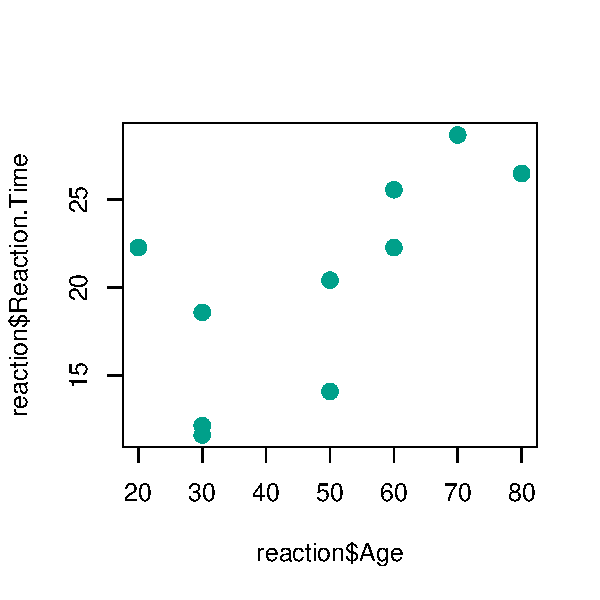
\includegraphics{inference_booklet_files/figure-latex/unnamed-chunk-3-1} \end{center}

\hypertarget{measures-of-dependence-and-the-simple-linear-model}{%
\section{Measures of Dependence and the Simple linear
model}\label{measures-of-dependence-and-the-simple-linear-model}}

\hypertarget{measuring-the-dependence}{%
\subsection{Measuring the dependence}\label{measuring-the-dependence}}

we define:

\begin{itemize}
\tightlist
\item
  \(X=Age\)\\
\item
  \(Y=Reaction.Time\)
\end{itemize}

We review some famous index to measure the (linear) dependence among two
variables

\hypertarget{covariance-and-variance}{%
\subsection{Covariance and Variance}\label{covariance-and-variance}}

\textbf{Covariance} between \(X\) and \(Y\):

\(\sigma_{xy}=\frac{\sum_{i=1} ^ n (x_i- \bar{x}) (y_i- \bar{y} )}{n}\)

\begin{itemize}
\tightlist
\item
  values between \(- \infty\) and \(\infty\)\\
\item
  \(\sigma_{xy} \approx 0\): there is no dependency between \(X\) and
  \(Y\)\\
\item
  \(\sigma_{xy} >> (<<) 0\): there is a strong positive (negative)
  dependency between \(X\) and \(Y\)
\end{itemize}

\begin{center}\rule{0.5\linewidth}{\linethickness}\end{center}

\textbf{Variance} of \(X\) (= covariance between \(X\) and \(X\)):

\(\sigma_{xx}=\sigma_{x} ^ 2= \frac{\sum_{i=1} ^ n (x_i- \bar{x}) ^ 2}{n}\)

\textbf{Standard Deviation} of \(X\):

\(\sigma_{xx}=\sqrt{\sigma_{xx}}=\sigma_{x}\)

\hypertarget{correlation}{%
\subsection{Correlation}\label{correlation}}

With the Covariance it is difficult to understand when the relationship
between \(X\) and \(Y\) is strong / weak. We note that

\(- \sigma_{x} \sigma_{y} \leq \sigma_{xy} \leq \sigma_{x} \sigma_{y}\)
is quivalent to
\(-1 \leq \frac{\sigma_{xy}}{\sigma_{x} \sigma_{y}} \leq 1\)

\textbf{Correlation} between \(X\) and \(Y\):

\(\rho_{xy}=\frac{\sigma{xy}}{\sigma_{x} \sigma_{y}} = \frac{\sum_{i=1} ^ n (x_i- \bar{x}) (y_i- \bar{y})}{\sqrt{\sum_{i=1} ^ n (x_i- \bar{ x}) ^ 2} \sqrt{\sum_{i=1} ^ n (y_i- \bar{y}) ^ 2}}\)

\begin{itemize}
\tightlist
\item
  values between \(-1\) and \(1\)
\item
  \(\rho_{xy} \approx 0\): there is no dependency between \(X\) and
  \(Y\)
\item
  \(\rho_{xy} \approx 1 (-1)\): there is a strong positive (negative)
  dependency between \(X\) and \(Y\)
\end{itemize}

\hypertarget{linear-trend-the-least-squares-method}{%
\subsection{Linear Trend, the least squares
method}\label{linear-trend-the-least-squares-method}}

We describe the relationship between\\
\texttt{Reaction.Time} and \texttt{Age} with a straight line.

\(Reaction.Time \approx \beta_0 + \beta_1 Age\)\\
\(Y=\beta_0 + \beta_1X\)

Let's draw a line `in the middle' of the data.

\begin{center}\rule{0.5\linewidth}{\linethickness}\end{center}

The \textbf{least-squares estimator}

We look for the one that passes more `in the middle', the one that
minimizes the sum of the squares of the residues:

\(\hat{\beta}_0\) and \(\hat{\beta}_1\) such that\\
\(\sum_{i=1} ^ n (y_i - (\hat{\beta}_0 + \hat{\beta}_1x_i )) ^ 2\) is
minimum.

\begin{center}\rule{0.5\linewidth}{\linethickness}\end{center}

Estimates:

\begin{itemize}
\tightlist
\item
  Angular coefficient:
  \(\hat{\beta}_1=\frac{\sigma_{xy}}{\sigma_{xx}}=\rho_{xy}\frac{\sigma_{y}}{\sigma_{x}}=\frac{\sum_{i=1}^n(x_i- \bar{x})(y_i-\bar{y})}{\sum_{i=1}^n (x_i-\bar{x})^2}=\)
  0.2064719\\
\item
  Intercept: \(\hat{\beta}_0=\bar{y}-\hat{\beta}_1\bar{x}=\) 10.3013483
\item
  Response (estimated \(y\)):
  \(\hat{y}_i=\hat{\beta}_0 + \hat{\beta}_1x_i\)
\item
  Residuals (from the estimated response):
  \(y_i - (\hat{\beta}_0 + \hat{\beta}_1 x_i)=y_i- \hat{y}_i\)
\end{itemize}

and therefore the least squares are the sum of the squared residuals:
\(\sum_{i=1} ^ n (y_i- \hat{\beta}_0 + \hat{\beta}_1x_i) ^ 2=\sum_{i=1} ^ n (y_i- \hat{y}_i ) ^ 2\)

\begin{center}\rule{0.5\linewidth}{\linethickness}\end{center}

A graphical representation:

\begin{Shaded}
\begin{Highlighting}[]
\NormalTok{model=}\KeywordTok{lm}\NormalTok{(Reaction.Time}\OperatorTok{~}\NormalTok{Age,}\DataTypeTok{data=}\NormalTok{reaction)}
\KeywordTok{coefficients}\NormalTok{(model)}
\end{Highlighting}
\end{Shaded}

\begin{verbatim}
## (Intercept)         Age 
##  10.3013483   0.2064719
\end{verbatim}

\begin{center}\rule{0.5\linewidth}{\linethickness}\end{center}

\begin{Shaded}
\begin{Highlighting}[]
\KeywordTok{plot}\NormalTok{(reaction}\OperatorTok{$}\NormalTok{Age,reaction}\OperatorTok{$}\NormalTok{Reaction.Time,}\DataTypeTok{pch=}\DecValTok{20}\NormalTok{,}\DataTypeTok{col=}\DecValTok{2}\NormalTok{,}\DataTypeTok{cex=}\DecValTok{1}\NormalTok{)}
\NormalTok{coeff=}\KeywordTok{round}\NormalTok{(}\KeywordTok{coefficients}\NormalTok{(model),}\DecValTok{1}\NormalTok{)}
\KeywordTok{title}\NormalTok{(}\KeywordTok{paste}\NormalTok{(}\StringTok{"Y="}\NormalTok{,coeff[}\DecValTok{1}\NormalTok{],}\StringTok{"+"}\NormalTok{,coeff[}\DecValTok{2}\NormalTok{],}\StringTok{"*X"}\NormalTok{))}
\KeywordTok{abline}\NormalTok{(model,}\DataTypeTok{col=}\DecValTok{1}\NormalTok{)}
\end{Highlighting}
\end{Shaded}

\begin{center}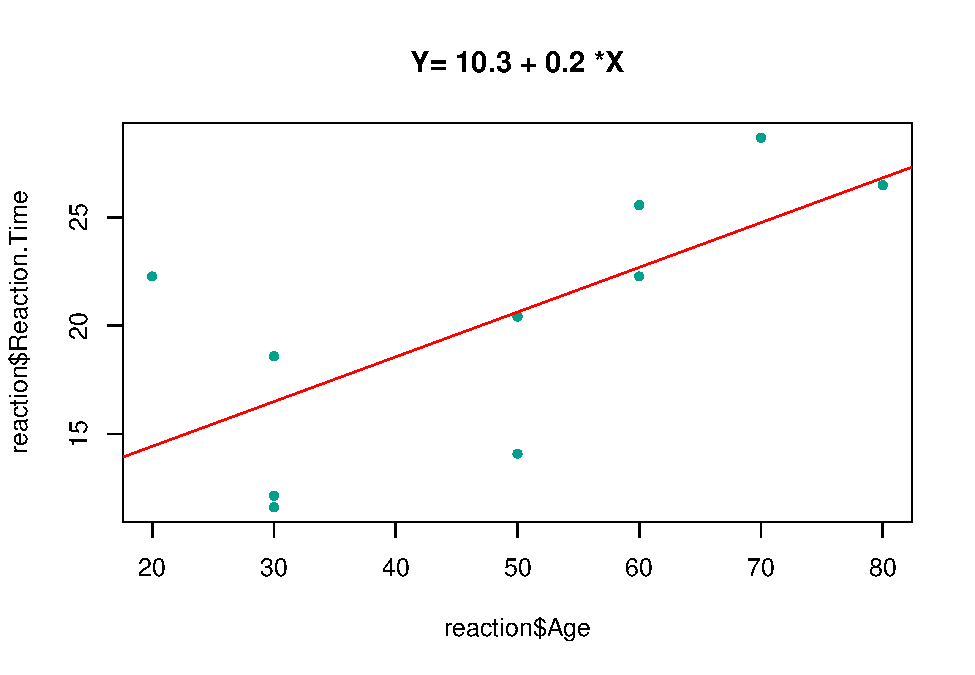
\includegraphics{inference_booklet_files/figure-latex/unnamed-chunk-6-1} \end{center}

\hypertarget{interpretation-of-the-coefficients}{%
\subsection{Interpretation of the
coefficients}\label{interpretation-of-the-coefficients}}

\begin{itemize}
\tightlist
\item
  \(\beta_0\) indicates the value of \(y\) when \(x=0\) (where the line
  intersects the ordinate axis).
\item
  \(\beta_1\) indicates how much \(y\) grows as a unit of \(x\) grows

  \begin{itemize}
  \tightlist
  \item
    If \(\beta_1=0\) there is no relation between \(x\) and
    \(y\).\(Y\)is constant (horizontal ), knowing\(x\)does not change
    the estimate of \(y\)
  \item
    If \(\beta_1> (<) 0\) the relation between \(x\) and \(y\) is
    positive (negative). When \(X\) passes from \(x\) a \(x + 1\) the
    estimate of \(Y\) changes from \(\hat{y}\) to
    \(\hat{y} + \hat{\beta}_1\)
  \end{itemize}
\end{itemize}

\hypertarget{permutation-approach-to-hypothesis-testing}{%
\section{Permutation approach to Hypothesis
Testing}\label{permutation-approach-to-hypothesis-testing}}

\hypertarget{some-remarks}{%
\subsection{Some remarks}\label{some-remarks}}

Let's note that all the measures above does not make any assumptions on
the random process that generate them.

Let's assume that \(Y\) - and possibly \(X\) - is not fix, while it is
generated by a random variable.

\begin{center}\rule{0.5\linewidth}{\linethickness}\end{center}

The question: \textbf{Is there a relationship between \(Y\) and \(X\)}?

We estimated \(\hat{\beta}_1=\) 0.2064719

but the \textbf{true value} \(\beta_1\) is really different from 0
(i.e.~no relationship)?\\
Otherwise, is the distance to 0 is due to the random sampling?

\begin{itemize}
\item
  \textbf{Null Hypothesis} \(H_0: \ \beta_1=0\) (the \textbf{true}
  \(\beta_1\), not its estimate \(\hat{\beta}_1\)!). There is no
  relationship between \(X\) and \(Y\).
\item
  \textbf{Alternative Hypothesis }\(H_1: \ \beta_1 >0\) The relationship
  is positive.
\end{itemize}

Other possible specifications of \(H_1: \ \beta_1< 0\) and, more
commonly, \(H_1: \ \beta_1 \neq 0\).

\hypertarget{permutation-tests---in-a-nutshell}{%
\subsection{Permutation tests - in a
nutshell}\label{permutation-tests---in-a-nutshell}}

As a toy example, let use a sub-set of the data:

\begin{verbatim}
##   Age Gender Reaction.Time
## 3  30      M         11.62
## 4  60      F         22.27
## 5  80      M         26.48
\end{verbatim}

\begin{center}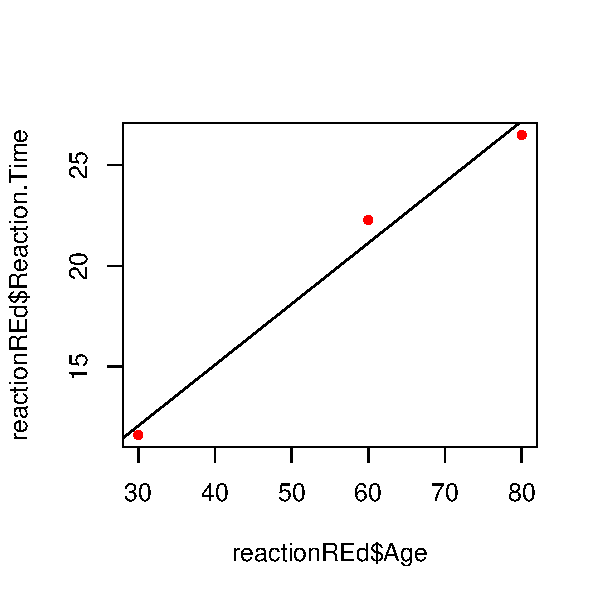
\includegraphics{inference_booklet_files/figure-latex/unnamed-chunk-7-1} \end{center}

\begin{center}\rule{0.5\linewidth}{\linethickness}\end{center}

\begin{itemize}
\tightlist
\item
  \emph{If \(H_0\)} is true: there is no linear relationship between
  \(X\) and \(Y\)
\item
  Therefore, the trend observed on the data is due to chance.
\item
  Any other match of \(x_i\) and \(y_i\) was equally likely to occur
\item
  I can generate the datasets of other hypothetical experiments by
  exchanging the order of the observations in \(Y\).
\item
  How many equally likely datasets could I get with\(X\) and
  \(Y\)observed? \(3 * 2 * 1=3!=6\) possible datasets.
\end{itemize}

Remark: Here we only assume that \(y\) is a random variable. The only
assumption here is the exchangeability of the observations: the joint
density \(f(y_1,\ldots,y_n)\) does not change when the ordering of
\(y_1,\ldots,y_n\) is changed.

\hypertarget{all-potential-datasets}{%
\subsection{All potential datasets}\label{all-potential-datasets}}

\begin{center}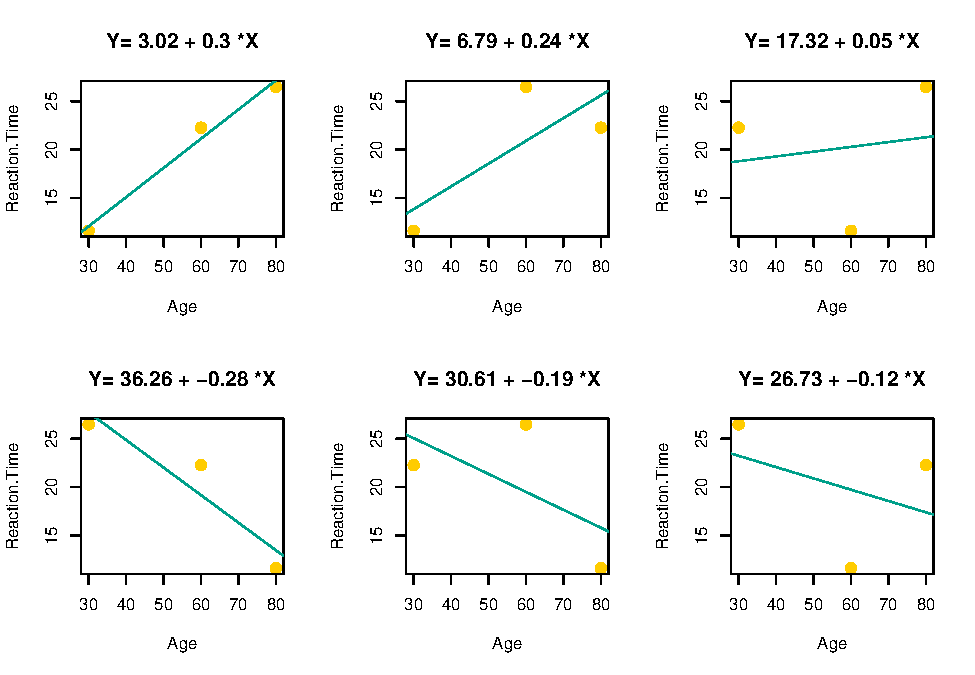
\includegraphics{inference_booklet_files/figure-latex/unnamed-chunk-8-1} \end{center}

\begin{center}\rule{0.5\linewidth}{\linethickness}\end{center}

\hypertarget{random-permutations}{%
\subsection{Random permutations}\label{random-permutations}}

In our data set, if we apply the same principle\ldots{}

How many permutations of the vector \(y_1,\ldots,y_n\) are possible?
\(n!=3628800\).

big, perhaps not too big \ldots{} but what happen with, for example,
\(n=20\)? We got \(20!=2.432902e+18\). This is too big, definitely!

We calculate a smaller (but sufficiently large) \(B\) of random
permutations.

here some example

\begin{center}\rule{0.5\linewidth}{\linethickness}\end{center}

\textbf{\texttt{Age} vs a permutations of \texttt{Reaction.Time}}

\begin{center}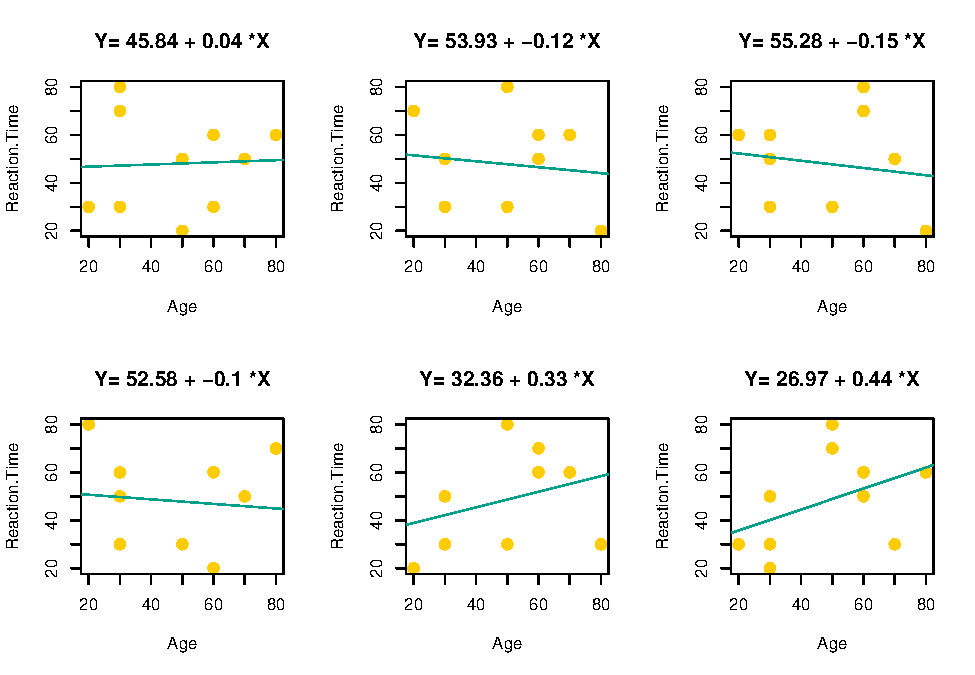
\includegraphics{inference_booklet_files/figure-latex/unnamed-chunk-9-1} \end{center}

\begin{center}\rule{0.5\linewidth}{\linethickness}\end{center}

We repeat \ensuremath{10^{4}} times and we look at the histogram of the
\(\hat{\beta}_1\)

\begin{Shaded}
\begin{Highlighting}[]
\CommentTok{# beta_1 estimated on the observed data:}
\NormalTok{beta1=}\KeywordTok{coefficients}\NormalTok{(}\KeywordTok{lm}\NormalTok{(Reaction.Time}\OperatorTok{~}\NormalTok{Age,}\DataTypeTok{data=}\NormalTok{reaction))[}\DecValTok{2}\NormalTok{]}

\CommentTok{# function that permutes the y values and calculates the coeff beta_1}
\NormalTok{my.beta.perm <-}\StringTok{ }\ControlFlowTok{function}\NormalTok{(Y,X)\{}
\NormalTok{  model=}\KeywordTok{lm}\NormalTok{(}\KeywordTok{sample}\NormalTok{(Y)}\OperatorTok{~}\NormalTok{X)}
  \KeywordTok{coefficients}\NormalTok{(model)[}\DecValTok{2}\NormalTok{]}
\NormalTok{\}}

\CommentTok{#replicate it B-1 times}
\NormalTok{beta.perm=}\StringTok{ }\KeywordTok{replicate}\NormalTok{(B,}\KeywordTok{my.beta.perm}\NormalTok{(reaction}\OperatorTok{$}\NormalTok{Reaction.Time, reaction}\OperatorTok{$}\NormalTok{Age ))}
\end{Highlighting}
\end{Shaded}

\begin{center}\rule{0.5\linewidth}{\linethickness}\end{center}

\begin{center}\includegraphics{inference_booklet_files/figure-latex/unnamed-chunk-11-1} \end{center}

\hypertarget{how-likely-hatbeta_1-obs-was}{%
\subsection{\texorpdfstring{How likely \(\hat{\beta}_1 ^{obs}\)
WAS?}{How likely \textbackslash hat\{\textbackslash beta\}\_1 \^{}\{obs\} WAS?}}\label{how-likely-hatbeta_1-obs-was}}

(before the experiment!)

How likely was it to get a \(\leq \hat{\beta}_1 ^{obs}\) value among the
many possible values of \(\hat{\beta}_1 ^{*b}\) (obtained by permuting
data)?

Remarks:

\begin{itemize}
\tightlist
\item
  \(\hat{\beta}_1 ^{* b}< \hat{\beta}_1 ^{obs}\) (closer to 0): less
  evidence against \(H_1\) than \(\hat{\beta}_1 ^{obs}\)
\item
  \(\hat{\beta}_1 ^{* b} \geq \hat{\beta}_1 ^{obs}\): equal or more
  evidence towards \(H_1\) than \(\hat{\beta}_1 ^{obs}\)
\end{itemize}

\hypertarget{calculation-of-the-p-value}{%
\subsection{Calculation of the
p-value}\label{calculation-of-the-p-value}}

Over B=\ensuremath{10^{4}} permutations we got 9822 times a
\(\hat{\beta}_1 ^{* b} \leq \hat{\beta}_1 ^{obs}\).

The p-value (significance) is
\(p=\frac{\# (\hat{\beta}_1 ^{* b} \geq \hat{\beta}_1 ^{obs})}{B + 1} =\)
0.018

\hypertarget{interpretation}{%
\subsection{Interpretation}\label{interpretation}}

The probability of \(p=P (\hat{\beta}_1 ^ * \leq \hat{\beta}_1=\) 0.206
\(| H_0)\) is equal to \(p =\) 0.018, i.e.~very small.\\
So, it was unlikely to get a value like this \textbf{IF \(H_0\) is
true}.

Neyman-Pearson's approach has made common the use of a significance
threshold for example \(\alpha=.05\) (or \(=. 01\)). When
\(p \leq \alpha\) rejects the hypothesis that there is no relationship
between X and Y (\(H_0\)). If so, we are inclined to think that \(H_1\)
is true (there is a positive relationship).

\begin{itemize}
\tightlist
\item
  Type I error: False Positive\\
  the true hypo is \(H_0\) (null correlation), BUT we accept \(H_1\)
  (correlation is positive)
\item
  Type II error: False Negative\\
  the true hypo is \(H_1\) (positive correlation), BUT we do not reject
  \(H_0\) (null correlation)
\end{itemize}

\begin{center}\rule{0.5\linewidth}{\linethickness}\end{center}

\textbf{Type I error control}

We want to guarantee not to get false relationships (a few false
positives), better to be conservative. To make this, we want to bound
the probability to make a false discovery:

\(P (p-value \leq \alpha | H_0) \leq \alpha\)

We built a machinery that in the long run (many replicates of the
experiment) finds false correlations with probability \(\alpha\)
(e.g.~\(0.05=5\%\)).

\hypertarget{we-make-it-in-flip}{%
\subsection{\texorpdfstring{We make it in
\texttt{flip}}{We make it in flip}}\label{we-make-it-in-flip}}

\begin{Shaded}
\begin{Highlighting}[]
\KeywordTok{library}\NormalTok{(flip)}

\NormalTok{(}\DataTypeTok{res=}\KeywordTok{flip}\NormalTok{(Reaction.Time}\OperatorTok{~}\NormalTok{Age,}\DataTypeTok{data=}\NormalTok{reaction,}
          \DataTypeTok{tail=}\DecValTok{1}\NormalTok{,}\DataTypeTok{perms =} \DecValTok{10000}\NormalTok{))}
\end{Highlighting}
\end{Shaded}

\begin{verbatim}
## 
##               Test  Stat tail p-value
## Reaction.Time    t 2.633    >  0.0158
\end{verbatim}

\begin{Shaded}
\begin{Highlighting}[]
\CommentTok{## compare also with}
\CommentTok{# flip(Reaction.Time~Age,data=reaction,tail=1,statTest = "cor")}
\CommentTok{# flip(Reaction.Time~Age,data=reaction,tail=1,statTest = "coeff")}
\end{Highlighting}
\end{Shaded}

\begin{center}\rule{0.5\linewidth}{\linethickness}\end{center}

\begin{Shaded}
\begin{Highlighting}[]
\KeywordTok{plot}\NormalTok{(res)}
\end{Highlighting}
\end{Shaded}

\begin{center}\includegraphics{inference_booklet_files/figure-latex/unnamed-chunk-13-1} \end{center}

\hypertarget{composite-alternatives-bilateral}{%
\subsection{Composite alternatives
(bilateral)}\label{composite-alternatives-bilateral}}

The hypothesis \(H_1: \ \beta_1 >0\) (the relation is positive) must be
justified with a priori knowledge.

More frequently, the Alternative hypothesis is appropriate:
\(H_1: \ \beta_1 \neq 0\) (there is a relationship, I do not assume the
direction)

I consider anomalous coefficients estimated as very small but also very
large (`far from 0'). The p-value is
\(p=\frac{\#(|\hat{\beta}_1^{*b} | \geq|\hat{\beta}_1^{obs}|)}{B+1}=\)
0.0345

\begin{center}\rule{0.5\linewidth}{\linethickness}\end{center}

In \texttt{flip}:

\begin{Shaded}
\begin{Highlighting}[]
\KeywordTok{library}\NormalTok{(flip)}
\NormalTok{(}\DataTypeTok{res=}\KeywordTok{flip}\NormalTok{(Reaction.Time}\OperatorTok{~}\NormalTok{Age,}\DataTypeTok{data=}\NormalTok{reaction,}\DataTypeTok{tail=}\DecValTok{0}\NormalTok{,}\DataTypeTok{perms=}\DecValTok{5000}\NormalTok{))}
\end{Highlighting}
\end{Shaded}

\begin{verbatim}
## 
##               Test  Stat tail p-value
## Reaction.Time    t 2.633   ><  0.0398
\end{verbatim}

\begin{center}\rule{0.5\linewidth}{\linethickness}\end{center}

\begin{Shaded}
\begin{Highlighting}[]
\KeywordTok{plot}\NormalTok{(res)}
\end{Highlighting}
\end{Shaded}

\begin{center}\includegraphics{inference_booklet_files/figure-latex/unnamed-chunk-15-1} \end{center}

\hypertarget{some-remarks-1}{%
\subsection{Some remarks}\label{some-remarks-1}}

\begin{itemize}
\tightlist
\item
  Do not be confused with bootstrap methods. The former are extractions
  without reintegration, the latter with. The former have almost optimal
  properties and have (almost always) an exact control of the first type
  errors.
\item
  A general approach and are applicable in many contexts. Very few
  assumptions.
\item
  Some dedicated R packages:

  \begin{itemize}
  \tightlist
  \item
    \href{http://cran.r-project.org/web/packages/flip/index.html}{flip}
    (the development version is on
    \href{https://github.com/livioivil/flip}{github})
  \item
    \href{http://cran.r-project.org/web/packages/coin/index.html}{coin}
  \item
    \href{https://cran.r-project.org/web/packages/permuco/index.html}{permuco}
  \end{itemize}
\item
  They are of limited applicability when there are many variables
  involved.
\end{itemize}

\hypertarget{parametric-linear-model}{%
\section{Parametric Linear Model}\label{parametric-linear-model}}

\hypertarget{from-permutation-tests-nonparametric-to-parametric-tests}{%
\subsection{From permutation tests (nonparametric) to parametric
tests}\label{from-permutation-tests-nonparametric-to-parametric-tests}}

We can see that the histogram of the statistical tests (calculated on
the permuted data) is well described by a \textbf{Gaussian }(normal)
curve.

\begin{center}\rule{0.5\linewidth}{\linethickness}\end{center}

\begin{Shaded}
\begin{Highlighting}[]
\KeywordTok{hist}\NormalTok{(beta.perm,}\DecValTok{50}\NormalTok{,}\DataTypeTok{probability=}\OtherTok{TRUE}\NormalTok{,}\DataTypeTok{col=}\DecValTok{2}\NormalTok{)}
\KeywordTok{curve}\NormalTok{(}\KeywordTok{dnorm}\NormalTok{(x,}\KeywordTok{mean}\NormalTok{(beta.perm),}\KeywordTok{sd}\NormalTok{(beta.perm)),}\DataTypeTok{add=}\OtherTok{TRUE}\NormalTok{,}\DataTypeTok{col=}\DecValTok{1}\NormalTok{,}\DataTypeTok{lwd=}\DecValTok{3}\NormalTok{)}
\KeywordTok{points}\NormalTok{(beta1,}\DecValTok{0}\NormalTok{,}\DataTypeTok{lwd=}\DecValTok{3}\NormalTok{,}\DataTypeTok{col=}\DecValTok{1}\NormalTok{)}
\end{Highlighting}
\end{Shaded}

\begin{center}\includegraphics{inference_booklet_files/figure-latex/unnamed-chunk-16-1} \end{center}

\hypertarget{the-simple-linear-model}{%
\subsection{The (simple) linear model}\label{the-simple-linear-model}}

We assume that the observed values are distributed around true values
\(\beta_0 + \beta_1 X\) according to a Gaussian law:

\(Y=\textrm{linear part} + \textrm{normal error}\)

\(Y=\beta_0 + \beta_1 X + \varepsilon\)

\textbf{Assumptions of the linear model }

\begin{itemize}
\tightlist
\item
  the \(\boldsymbol{y_i=\beta_0 + \beta_1 x_i + \varepsilon_i}\) the
  relationship between \(X\) and the true (mean) \(Y\) is linear.
\item
  the \textbf{observations } are \textbf{independent} each others (
  knowing the value of the \(y_i\)observation does not help me to
  predict the value of \(y_{i + 1}\)). The random part is
  \(\varepsilon_i\), these are the independent terms.
\item
  \(\boldsymbol{\varepsilon_i \sim N (0, \sigma ^ 2), \ \forall i=1, \ldots, n}\)
  errors have normal distribution with zero mean and common variance
  (homoschedasticity: same variance).
\end{itemize}

\hypertarget{hypothesis-testing}{%
\subsection{Hypothesis testing}\label{hypothesis-testing}}

If these assumptions are true,

\(\hat{\beta_1} \sim N (\beta_1, \sigma ^ 2 / \sum (x_i- \bar{x}) ^ 2)\)

We calculate the test statistic:

\(t=\frac{\hat{\beta_1}}{std.dev\ \hat{\beta_1}}=\frac{\hat{\beta_1}}{\sqrt{\sum_{i=1} ^ n (y_i- \hat{y}_i) ^ 2 / \sum (x_i- \bar{x}) ^ 2 / (n-2)}}\)

If \(H_0: \beta_1=0\), \(t \sim t (n-2)\) is true

On \texttt{reaction} data and \(H_1: \beta_1 \neq 0\) (bilateral
alternative)

\begin{center}\rule{0.5\linewidth}{\linethickness}\end{center}

\begin{Shaded}
\begin{Highlighting}[]
\NormalTok{model=}\KeywordTok{lm}\NormalTok{ (Reaction.Time }\OperatorTok{~}\StringTok{ }\NormalTok{Age, }\DataTypeTok{data=}\NormalTok{reaction)}
\KeywordTok{summary}\NormalTok{(model) }\OperatorTok{$}\StringTok{ }\NormalTok{coefficients}
\end{Highlighting}
\end{Shaded}

\begin{verbatim}
##               Estimate Std. Error  t value   Pr(>|t|)
## (Intercept) 10.3013483 4.04406774 2.547274 0.03431997
## Age          0.2064719 0.07841111 2.633197 0.03002876
\end{verbatim}

Similar result, but much more assumptions!

\hypertarget{power-is-nothing-without-control}{%
\subsection{Power is nothing without
control}\label{power-is-nothing-without-control}}

We don't know if the data are genareted under \(H_0\) or under \(H_1\).

But we have a tool (the test) that

\begin{itemize}
\tightlist
\item
  if the data are generated \textbf{under \(H_0\)}: it suggests (wrong)
  \(H_1\) (i.e.~\(p\leq \alpha\), type I error, false positive) with
  probability \(\alpha\). E.g. \(\alpha=.05\), low probability.
\item
  if the data are generated \textbf{under \(H_1\)}: it suggests
  (correct) \(H_1\) (i.e.~true positive) with probability larger than
  \(\alpha\).\\
  This is the Power of a test. The Power is unknown, but we hope it is
  as high as possible.
\end{itemize}

\hypertarget{terminology}{%
\subsection{Terminology}\label{terminology}}

\begin{itemize}
\item
  Probability of \textbf{Type I error} (Probability of \textbf{False
  Positive}, \(\alpha\)): the probability to find a relationship when it
  does not exist (true \(H_0\), the test judges \(H_1\)).
\item
  Probability of \textbf{Type II error} (Probability of \textbf{False
  Negative}): the probability NOT to find a relationship when it does
  exist (true \(H_1\), the test judges \(H_0\)).
\item
  \textbf{Specificity}: the probability NOT to find a relationship when
  it does NOT exist (true \(H_0\), the test judges \(H_0\)). it is equal
  to 1 - Type I error.
\item
  \textbf{Power} (\textbf{Sensitivity}): the probability to NOT find a
  relationship when it does exist (true \(H_1\), the test judges
  \(H_1\)). it is equal to 1 - Type II error.
\end{itemize}

\hypertarget{properties}{%
\subsection{Properties}\label{properties}}

If the parametric assumptions are valid, the test guarantes

\begin{itemize}
\tightlist
\item
  the control of the type I error at the \(\alpha\) level,\\
\item
  the maximum power (minimum error of type II \(\beta\)) among all the
  possible tests,\\
\item
  asymptotic consistency (if they are under \(H_1\) rejection always for
  sufficiently large \(n\)).
\end{itemize}

The permutation tests usually have slightly less power and converge to
the corresponding parametric tests, IF they exist.

\hypertarget{confidence-intervals}{%
\subsection{Confidence intervals}\label{confidence-intervals}}

The parametric approach also allows us to calculate confidence intervals

\begin{Shaded}
\begin{Highlighting}[]
\KeywordTok{confint}\NormalTok{(model)}
\end{Highlighting}
\end{Shaded}

\begin{verbatim}
##                  2.5 %     97.5 %
## (Intercept) 0.97571138 19.6269853
## Age         0.02565557  0.3872883
\end{verbatim}

In linear model:
\[C.I.= [ \hat{\beta_1}-t_{1-\alpha/2} \hat{\sigma}/\sqrt{n}, \hat{\beta_1}+t_{1-\alpha/2} \hat{\sigma}/\sqrt{n}]\]
(\(t_{1-\alpha/2}\) is the threshold given by a t-distribution with CDF
equal to \(1-\alpha/2\) and d.f. \(n-1\))

Confidence intervals are constructed in such a way that in the long run
they include the true value \(\beta_1\) with probability \(1-\alpha\)
(e.g.~95 \%).

\begin{center}\rule{0.5\linewidth}{\linethickness}\end{center}

Once the data has been collected, the Conf Int is computed.\\
It will includes or not the true value \(\beta_1\).\\
We only have the certificate of quality of out test, Conf Int in the
95\% of the (previous) cases was wrong 95\% of the times.

Confidence intervals and hypothesis testing are closely related: if a
confidence interval at level \(1-\alpha\) does not include the 0, the
p-value that tests \(H_0:\ \beta_1 = 0\) will be \(p<\alpha\).

\hypertarget{a-simulation-to-better-understand}{%
\section{A simulation to better
understand}\label{a-simulation-to-better-understand}}

\hypertarget{a-single-fictitious-dataset}{%
\subsection{A single fictitious
dataset}\label{a-single-fictitious-dataset}}

We generate a fictitious datasets and see how the tests and confidence
intervals behave.

\begin{itemize}
\tightlist
\item
  use the observed values for \(Age\) in the original dataset\\
\item
  randomly generate values for \(Reaction.Time\).
\item
  get the statistics (p-values, confidence interval)
\end{itemize}

\hypertarget{h_0-is-true-type-i-error-control}{%
\subsection{\texorpdfstring{\(H_0\) is true (Type I error
control)}{H\_0 is true (Type I error control)}}\label{h_0-is-true-type-i-error-control}}

There is no relationship between \(Age\) and \(Reaction.Time\).

then: \(Reaction.Time=\beta_0 + 0 Age + \varepsilon\)

\(\varepsilon\) can be assumed to be normal \(N(0,\sigma^2)\).

How to set \(\beta_0\) and \(\sigma^2\)?\\
As reasonable values, we can use mean and variance calculated on the
sample:

\begin{Shaded}
\begin{Highlighting}[]
\NormalTok{m=}\KeywordTok{mean}\NormalTok{(reaction}\OperatorTok{$}\NormalTok{Reaction.Time)}
\NormalTok{s2=}\KeywordTok{var}\NormalTok{(reaction}\OperatorTok{$}\NormalTok{Reaction.Time)}
\NormalTok{s=}\KeywordTok{sqrt}\NormalTok{(s2)}
\NormalTok{n=}\KeywordTok{length}\NormalTok{(reaction}\OperatorTok{$}\NormalTok{Age)}
\end{Highlighting}
\end{Shaded}

\begin{itemize}
\tightlist
\item
  \(\beta_0=m=\) \texttt{m=} 20.212
\item
  \(\sigma=\) \texttt{s=} 6.0265041
\end{itemize}

\begin{center}\rule{0.5\linewidth}{\linethickness}\end{center}

\begin{Shaded}
\begin{Highlighting}[]
\CommentTok{# generate random Reaction.Time}
\NormalTok{Reaction.Time=}\KeywordTok{rnorm}\NormalTok{(n,m,s) }\CommentTok{# equivalent to m+rnorm(n,0,s)}
\CommentTok{#and fit the model}
\NormalTok{mod=}\KeywordTok{lm}\NormalTok{(Reaction.Time}\OperatorTok{~}\NormalTok{reaction}\OperatorTok{$}\NormalTok{Age)}
\KeywordTok{summary}\NormalTok{(mod)}\OperatorTok{$}\NormalTok{coefficients}
\end{Highlighting}
\end{Shaded}

\begin{verbatim}
##                Estimate Std. Error   t value    Pr(>|t|)
## (Intercept)  25.9745219  5.5037753  4.719401 0.001503326
## reaction$Age -0.1076552  0.1067136 -1.008823 0.342594709
\end{verbatim}

\begin{Shaded}
\begin{Highlighting}[]
\KeywordTok{confint}\NormalTok{(mod)}
\end{Highlighting}
\end{Shaded}

\begin{verbatim}
##                   2.5 %     97.5 %
## (Intercept)  13.2827934 38.6662505
## reaction$Age -0.3537373  0.1384269
\end{verbatim}

\hypertarget{many-datasets}{%
\subsection{Many datasets}\label{many-datasets}}

Now we generate many (e.g.~1000) datasets and we store the p-values.

\begin{Shaded}
\begin{Highlighting}[]
\NormalTok{sim <-}\StringTok{ }\ControlFlowTok{function}\NormalTok{(Age,n,m,s)\{}
\NormalTok{  Reaction.Time=}\KeywordTok{rnorm}\NormalTok{(n,m,s)}
  \CommentTok{#get the p-value from the output}
  \KeywordTok{summary}\NormalTok{(}\KeywordTok{lm}\NormalTok{(Reaction.Time}\OperatorTok{~}\NormalTok{Age))}\OperatorTok{$}\NormalTok{coefficients[}\StringTok{"Age"}\NormalTok{,}\StringTok{"Pr(>|t|)"}\NormalTok{]}
\NormalTok{\}}

\NormalTok{p.sim=}\KeywordTok{replicate}\NormalTok{(}\DecValTok{1000}\NormalTok{,}\KeywordTok{sim}\NormalTok{(reaction}\OperatorTok{$}\NormalTok{Age,n,m,s))}
\end{Highlighting}
\end{Shaded}

\begin{itemize}
\tightlist
\item
  What do I expect the distribution of these p-values to be?
\item
  If I plot a histogram, what do I expect?
\item
  What will be the proportion of p-values \(\leq 0.05\)?
\end{itemize}

\begin{center}\rule{0.5\linewidth}{\linethickness}\end{center}

\begin{Shaded}
\begin{Highlighting}[]
\KeywordTok{hist}\NormalTok{(p.sim)}
\end{Highlighting}
\end{Shaded}

\begin{center}\includegraphics{inference_booklet_files/figure-latex/unnamed-chunk-22-1} \end{center}

\begin{center}\rule{0.5\linewidth}{\linethickness}\end{center}

\begin{Shaded}
\begin{Highlighting}[]
\CommentTok{#how many p<.05}
\KeywordTok{sum}\NormalTok{(p.sim}\OperatorTok{<}\NormalTok{.}\DecValTok{05}\NormalTok{)}
\end{Highlighting}
\end{Shaded}

\begin{verbatim}
## [1] 51
\end{verbatim}

\begin{Shaded}
\begin{Highlighting}[]
\CommentTok{#proportion of p<.05}
\KeywordTok{mean}\NormalTok{(p.sim}\OperatorTok{<}\NormalTok{.}\DecValTok{05}\NormalTok{)}
\end{Highlighting}
\end{Shaded}

\begin{verbatim}
## [1] 0.051
\end{verbatim}

\begin{center}\rule{0.5\linewidth}{\linethickness}\end{center}

Now the (empirical) cumulative distribution

\begin{Shaded}
\begin{Highlighting}[]
\KeywordTok{plot}\NormalTok{(}\KeywordTok{ecdf}\NormalTok{(p.sim),}\DataTypeTok{xlab=}\StringTok{"alpha"}\NormalTok{,}\DataTypeTok{ylab=}\StringTok{"Empirical Type I error"}\NormalTok{, }\DataTypeTok{col=}\DecValTok{1}\NormalTok{,}\DataTypeTok{main=}\StringTok{"Type I error as a function of alpha"}\NormalTok{,}\DataTypeTok{lwd=}\DecValTok{3}\NormalTok{,}\DataTypeTok{asp=}\DecValTok{1}\NormalTok{)}
\KeywordTok{abline}\NormalTok{(}\DecValTok{0}\NormalTok{,}\DecValTok{1}\NormalTok{,}\DataTypeTok{col=}\DecValTok{2}\NormalTok{)}
\end{Highlighting}
\end{Shaded}

\begin{center}\includegraphics{inference_booklet_files/figure-latex/unnamed-chunk-24-1} \end{center}

For each value of the abscissa \(\alpha\) we see the empirical estimate
of the type I error.

For any given \(\alpha\), the estimated proportion is around \(\alpha\)
(and would converge to \(\alpha\) if we increases the number of
replications)

Very good!! :)

\hypertarget{h_1-is-true-power-evaluation}{%
\subsection{\texorpdfstring{\(H_1\) is true (Power
evaluation)}{H\_1 is true (Power evaluation)}}\label{h_1-is-true-power-evaluation}}

There is a relationship between \(Age\) and \(Reaction.Time\). I can use
use the linear normal model with parameters - just an example -
calculated on the sample.

\begin{Shaded}
\begin{Highlighting}[]
\NormalTok{modelF=}\KeywordTok{lm}\NormalTok{(Reaction.Time}\OperatorTok{~}\NormalTok{Age,}\DataTypeTok{data=}\NormalTok{reaction)}
\KeywordTok{coefficients}\NormalTok{(modelF)}
\end{Highlighting}
\end{Shaded}

\begin{verbatim}
## (Intercept)         Age 
##  10.3013483   0.2064719
\end{verbatim}

\begin{Shaded}
\begin{Highlighting}[]
\NormalTok{beta0=}\KeywordTok{coefficients}\NormalTok{(modelF)[}\DecValTok{1}\NormalTok{]}
\NormalTok{beta1=}\KeywordTok{coefficients}\NormalTok{(modelF)[}\DecValTok{2}\NormalTok{]}
\end{Highlighting}
\end{Shaded}

\begin{center}\rule{0.5\linewidth}{\linethickness}\end{center}

\begin{Shaded}
\begin{Highlighting}[]
\NormalTok{y_linear_part=beta0}\OperatorTok{+}\NormalTok{beta1}\OperatorTok{*}\NormalTok{reaction}\OperatorTok{$}\NormalTok{Age }
\NormalTok{s=}\KeywordTok{sd}\NormalTok{(}\KeywordTok{residuals}\NormalTok{(modelF))}
\NormalTok{n=}\KeywordTok{length}\NormalTok{(reaction}\OperatorTok{$}\NormalTok{Age)}

\CommentTok{# generate random Reaction.Time}
\NormalTok{Reaction.Time=y_linear_part}\OperatorTok{+}\KeywordTok{rnorm}\NormalTok{(n,}\DecValTok{0}\NormalTok{,s)}
\CommentTok{#fit the model (estimate the parameters)}
\KeywordTok{summary}\NormalTok{(}\KeywordTok{lm}\NormalTok{(Reaction.Time}\OperatorTok{~}\NormalTok{Age,}\DataTypeTok{data=}\NormalTok{reaction))}\OperatorTok{$}\NormalTok{coefficients}
\end{Highlighting}
\end{Shaded}

\begin{verbatim}
##               Estimate Std. Error  t value   Pr(>|t|)
## (Intercept) 10.3013483 4.04406774 2.547274 0.03431997
## Age          0.2064719 0.07841111 2.633197 0.03002876
\end{verbatim}

\hypertarget{many-datasets-1}{%
\subsection{Many datasets}\label{many-datasets-1}}

Now we generate many (e.g.~1000) datasets and, for each, we store the
p-value.

\begin{Shaded}
\begin{Highlighting}[]
\NormalTok{p.sim=}\KeywordTok{replicate}\NormalTok{(}\DecValTok{1000}\NormalTok{,}\KeywordTok{sim}\NormalTok{(reaction}\OperatorTok{$}\NormalTok{Age,n,y_linear_part,s))}
\end{Highlighting}
\end{Shaded}

\begin{itemize}
\tightlist
\item
  What do I expect the distribution of these p-values to be?
\item
  If I plot a histogram, what do I expect?
\item
  What will be the proportion of p-values \(\leq 0.05\)?
\end{itemize}

\begin{center}\rule{0.5\linewidth}{\linethickness}\end{center}

\begin{Shaded}
\begin{Highlighting}[]
\KeywordTok{hist}\NormalTok{(p.sim)}
\end{Highlighting}
\end{Shaded}

\begin{center}\includegraphics{inference_booklet_files/figure-latex/unnamed-chunk-28-1} \end{center}

\begin{center}\rule{0.5\linewidth}{\linethickness}\end{center}

\begin{Shaded}
\begin{Highlighting}[]
\CommentTok{#how many p<.05}
\KeywordTok{sum}\NormalTok{(p.sim}\OperatorTok{<}\NormalTok{.}\DecValTok{05}\NormalTok{)}
\end{Highlighting}
\end{Shaded}

\begin{verbatim}
## [1] 678
\end{verbatim}

\begin{Shaded}
\begin{Highlighting}[]
\CommentTok{#proportion of p<.05}
\KeywordTok{mean}\NormalTok{(p.sim}\OperatorTok{<}\NormalTok{.}\DecValTok{05}\NormalTok{)}
\end{Highlighting}
\end{Shaded}

\begin{verbatim}
## [1] 0.678
\end{verbatim}

\begin{center}\rule{0.5\linewidth}{\linethickness}\end{center}

Now the (empirical) cumulative distribution

\begin{Shaded}
\begin{Highlighting}[]
\KeywordTok{plot}\NormalTok{(}\KeywordTok{ecdf}\NormalTok{(p.sim),}\DataTypeTok{xlab=}\StringTok{"alpha"}\NormalTok{,}\DataTypeTok{ylab=}\StringTok{"Empirical Power"}\NormalTok{, }\DataTypeTok{col=}\DecValTok{1}\NormalTok{,}\DataTypeTok{main=}\StringTok{"Power as a function of alpha"}\NormalTok{,}\DataTypeTok{lwd=}\DecValTok{3}\NormalTok{,}\DataTypeTok{asp=}\DecValTok{1}\NormalTok{)}
\KeywordTok{abline}\NormalTok{(}\DecValTok{0}\NormalTok{,}\DecValTok{1}\NormalTok{,}\DataTypeTok{col=}\DecValTok{2}\NormalTok{)}
\end{Highlighting}
\end{Shaded}

\begin{center}\includegraphics{inference_booklet_files/figure-latex/unnamed-chunk-30-1} \end{center}

For each value of the abscissa \(\alpha\) we see the empirical estimate
of the Power.

For any given \(\alpha\), the estimated proportion greater than
\(\alpha\), the test has power!

Very good!! :)

\hypertarget{homework-1-effect-of-measure-quality-noise}{%
\subsection{Homework 1: Effect of measure quality
(noise)}\label{homework-1-effect-of-measure-quality-noise}}

\begin{enumerate}
\def\labelenumi{\arabic{enumi}.}
\item
  How do the Type I error varies as a function of the standard deviation
  of the normal errors?\\
  Hint: Simulate with different sd (e.g.~2,4,8,16), store the proportion
  of rejections for \(\alpha=.05\), plot the sd vs rejections.
\item
  Same task, but under \(H_1\) (power study)
\end{enumerate}

\hypertarget{solution}{%
\subsection{Solution}\label{solution}}

\begin{center}\rule{0.5\linewidth}{\linethickness}\end{center}

\begin{center}\rule{0.5\linewidth}{\linethickness}\end{center}

\hypertarget{homework-2-effect-of-sample-size}{%
\subsection{Homework 2: Effect of sample
size}\label{homework-2-effect-of-sample-size}}

\begin{enumerate}
\def\labelenumi{\arabic{enumi}.}
\item
  How does the type I error varies as a function of the sample size?
  (Same hint of homework 1, but here you sample \texttt{Age} \texttt{n}
  times and compute \texttt{y\_linear\_part} )
\item
  How does the power?
\end{enumerate}

\hypertarget{solution-1}{%
\subsection{Solution}\label{solution-1}}

\begin{center}\rule{0.5\linewidth}{\linethickness}\end{center}

\hypertarget{h0}{%
\subsubsection{H0}\label{h0}}

\begin{center}\rule{0.5\linewidth}{\linethickness}\end{center}

\hypertarget{h1}{%
\subsubsection{H1}\label{h1}}

\hypertarget{homework-3-confidence-intervals}{%
\subsection{Homework 3: Confidence
intervals}\label{homework-3-confidence-intervals}}

Make similar evaluations of Homework 1 and 2 for confidence intervals:

\begin{itemize}
\tightlist
\item
  set \(\alpha=.05\),
\item
  genate datasets, fit the models,
\item
  Two quantities are of interest here:

  \begin{itemize}
  \tightlist
  \item
    counts of times the confidence interval contains the TRUE value
    \(\beta_1\)
  \item
    length of the confidence interval
  \end{itemize}
\end{itemize}

\hypertarget{solution-sigma-noise}{%
\subsection{Solution: Sigma (noise)}\label{solution-sigma-noise}}

\begin{center}\rule{0.5\linewidth}{\linethickness}\end{center}

\hypertarget{h0-1}{%
\subsubsection{H0}\label{h0-1}}

\begin{center}\rule{0.5\linewidth}{\linethickness}\end{center}

\hypertarget{h1-1}{%
\subsubsection{H1}\label{h1-1}}

\hypertarget{solution-sample-size}{%
\subsection{Solution: sample size}\label{solution-sample-size}}

\begin{center}\rule{0.5\linewidth}{\linethickness}\end{center}

\hypertarget{h0-2}{%
\subsubsection{H0}\label{h0-2}}

\begin{center}\rule{0.5\linewidth}{\linethickness}\end{center}

\hypertarget{h1-2}{%
\subsubsection{H1}\label{h1-2}}


\end{document}
